\newcommand{\hascwidth}{.49\textwidth}
\subsection{Home Assistant}
\label{sec:home-assistant}

Bei Home Assistant handelt es sich um Open Source Software im Bereich Smart Home. Es zielt darauf ab, die Privatsphäre der Nutzenden zu erhöhen, indem so weit wie möglich auf externe Server verzichtet wird\parencite{openhomefoundationHomeAssistant}. Typischerweise wird Home Assistant auf einem Raspberry Pi betrieben, der sich in der gleichen Wohneinheit mit den zu kontrollierenden Geräten befindet.

Im Folgenden werden die wichtigsten Konzepte für das Verständnis von Home Assistant vorgestellt. \textbf{Integrationen} stellen Software dar, welche mit anderen Plattformen kommuniziert, und es somit ermöglicht, Geräte von verschiedenen Herstellern einzubinden. Daraufhin sind diese als \textbf{Geräte} in Home Assistant vertreten und stellen sogenannte \textbf{Entitäten} bereit, welche den Zustand des Geräts beschreiben und kontrollieren. Auf Basis von Sensoren und Kontroll-Entitäten können nun \textbf{Automatisierungen} erstellt werden. Diese bestehen aus \textbf{Auslösern}, welche die Automatisierung starten und etwas beschreiben, was im Haus passiert (Beispiel: "Person betritt Wohnzimmer."). Des Weiteren können \textbf{Bedingungen} angegeben werden, die zusätzliche Tests darstellen, welche die Ausführung der Automatisierung verhindern können (Beispiel: "Umgebungslicht ist unter 20 Lux."). Sobald die Automatisierung ausgelöst wurde und die Bedingungen übereinstimmen, werden \textbf{Aktionen} ausgeführt. Diese steuern Geräte oder Entitäten und werden standardmäßig als Liste ausgeführt (Beispiel: "Leselampe anschalten, Musik abspielen."). \textbf{Skripte} sind Sammlungen von Aktionen, welche als eine Aktion wiederverwendet werden können \parencite{openhomefoundationConceptsTerminology}.

Sowohl Automatisierungen als auch Skripte werden als \ac{YAML}-Dateien gespeichert und können über einen visuellen Editor bearbeitet werden. Dieser wird im Folgenden betrachtet.

\subsubsection{Editor zum Erstellen von Automatisierungen}
Abbildung \ref{fig:hassio-automation-empty} zeigt den Initialzustand bei der Erstellung einer neuen Automatisierung. Die Ansicht ist in drei Abschnitte unterteilt, in der die drei relevanten Bausteine angegeben werden können. Abschnitte, die noch keinen Baustein enthalten, verfügen über einen Button zum Hinzufügen dieser. Der Button öffnet ein kontextabhängiges Pop-up-Fenster, wie in Abbildung \ref{fig:hassio-automation-trigger-select-2} zu sehen ist. Je nach Typ des Bausteins werden dort unterschiedliche Elemente angezeigt. So werden im Auswahlmenü für Auslöser (Abbildung \ref{fig:hassio-automation-trigger-select-2}) nur Auslöser gezeigt. In diesem Falle können Auslöser die Zustände von Geräten oder Entitäten, sowie zeitliche und örtlich bedingte Zustände sein.

\begin{figure}[!ht]
  \begin{minipage}[t]{\hascwidth}
    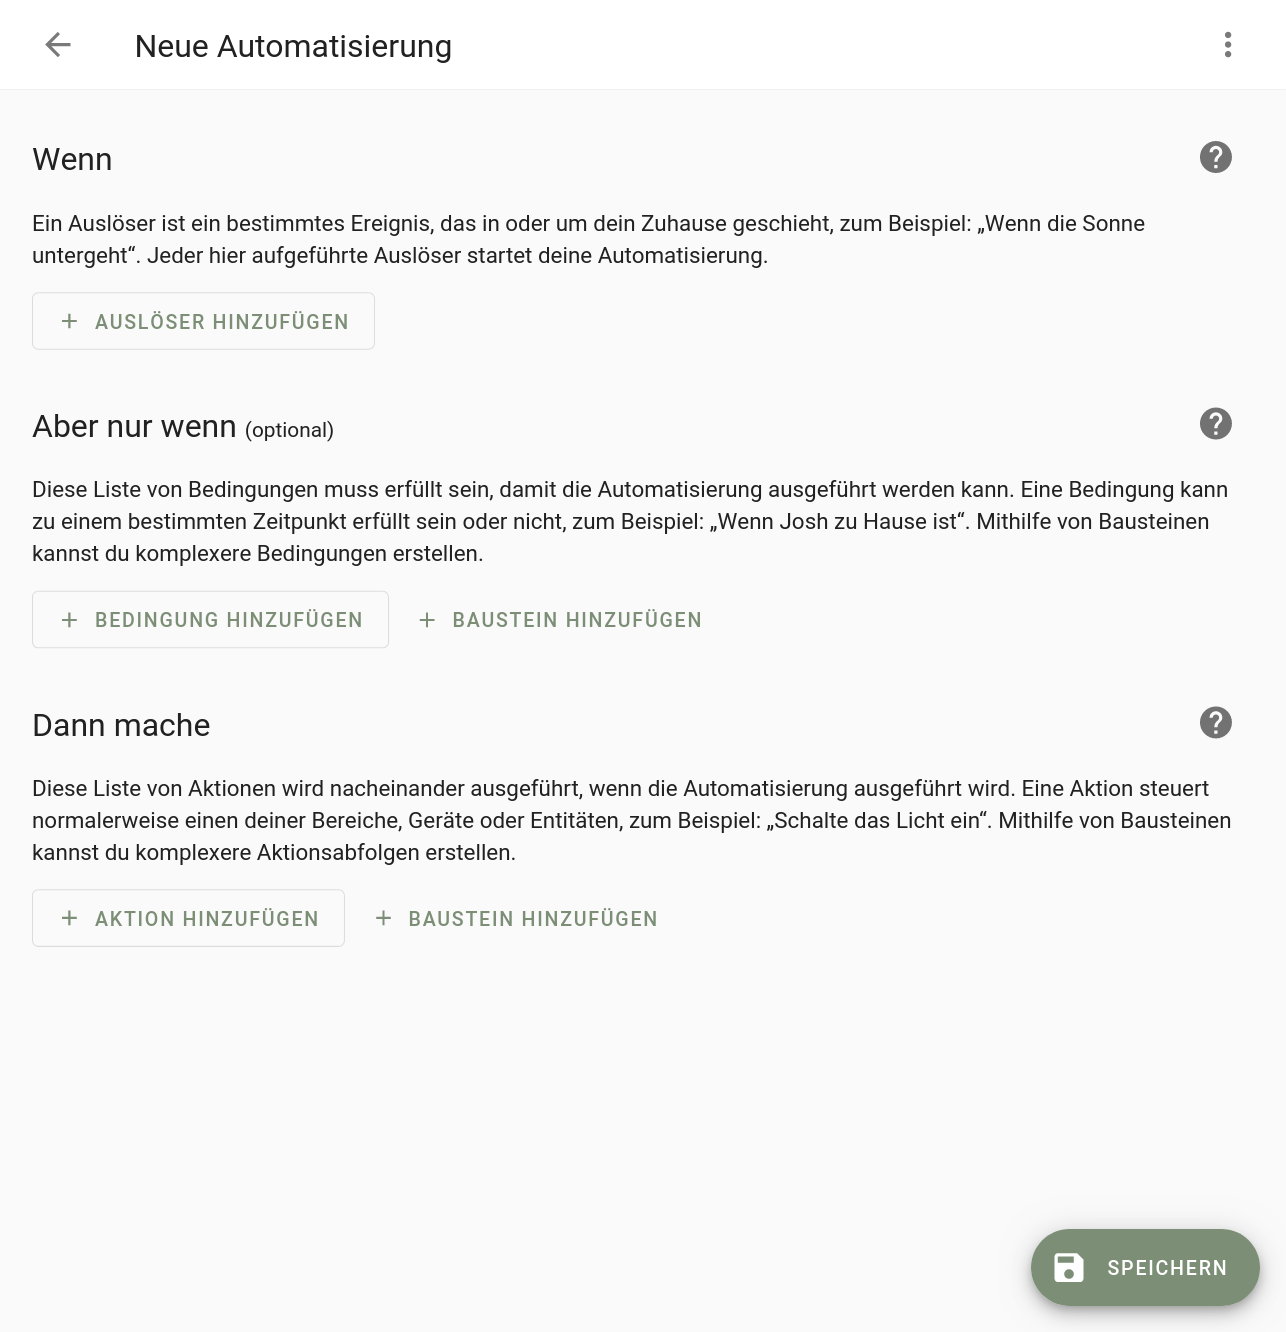
\includegraphics[width=\linewidth]{assets/hassio-automation-empty.png}
    \caption[Erstellung einer Automatisierung in Home Assistant]{Startpunkt der Erstellung einer Automatisierung in Home Assistant. Die Ansicht besteht aus drei Bereichen für Auslöser, Bedingungen und Aktionen, unter denen korrespondierende Blöcke hinzugefügt werden können.}
    \label{fig:hassio-automation-empty}
  \end{minipage}
  \hfill
  \begin{minipage}[t]{\hascwidth}
    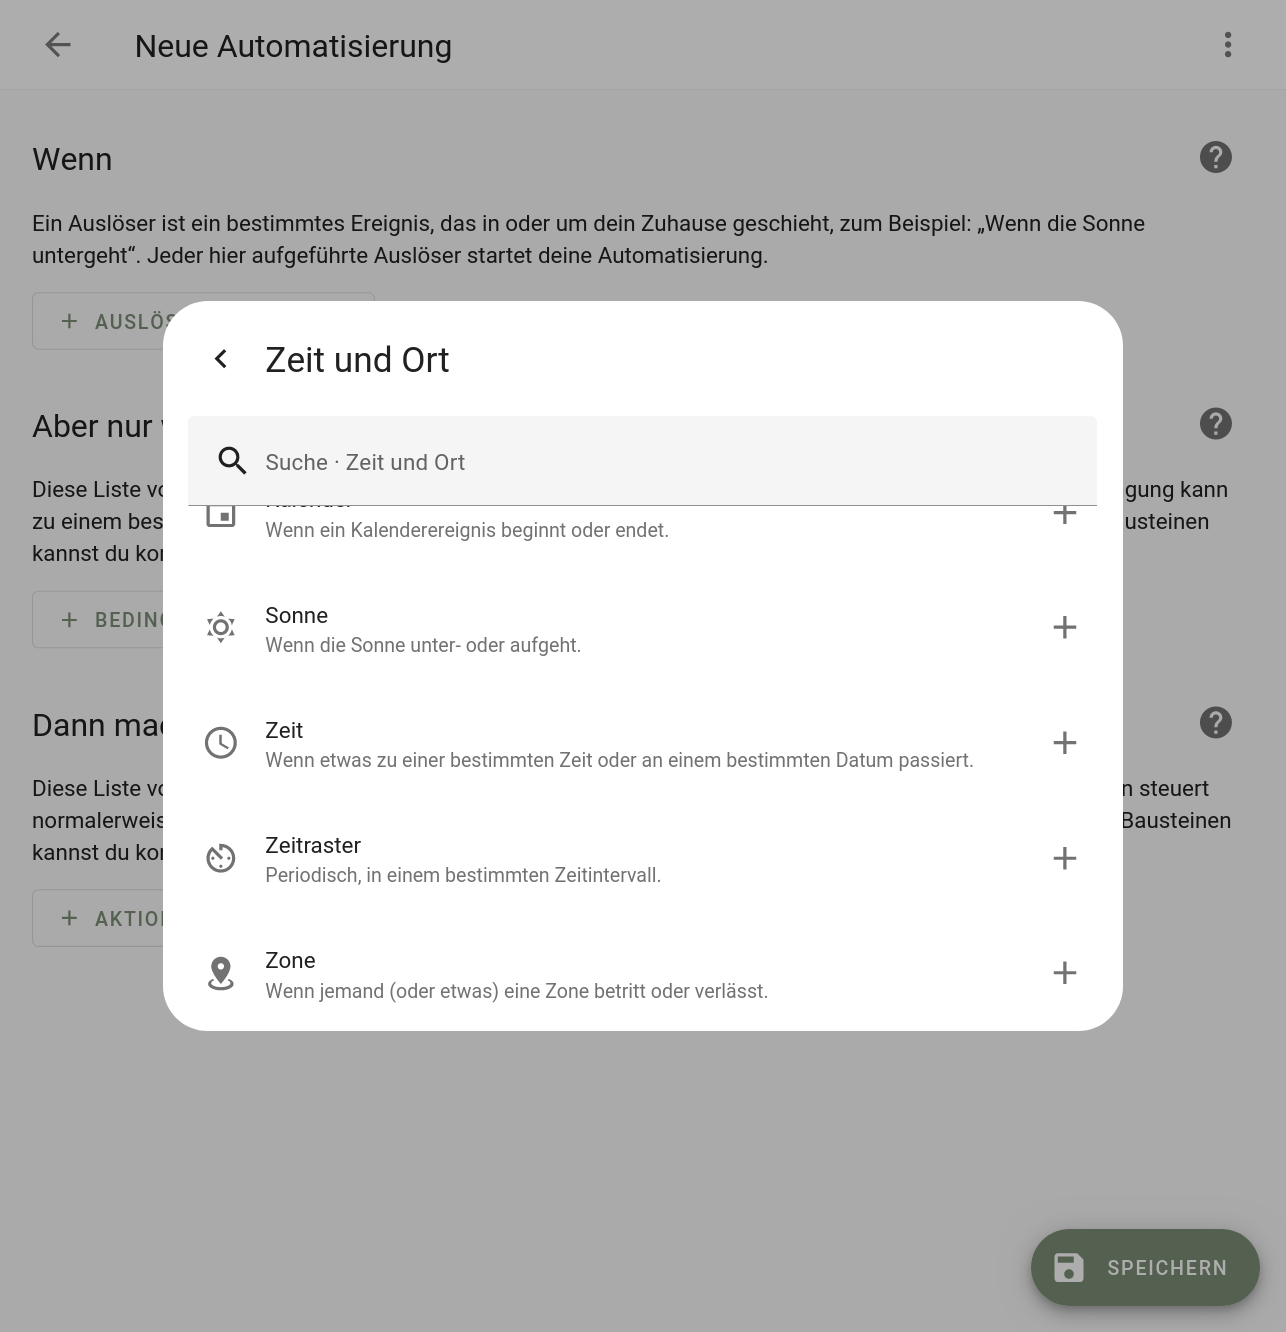
\includegraphics[width=\linewidth]{assets/hassio-automation-trigger-select-2.png}
    \caption[Auswahl eines Auslösers in Home Assistant]{Auswahl eines Auslösers. Gezeigt wird ein Untermenü der Kategorie "Zeit und Ort", welche zuvor ausgewählt wurde. Die hier verfügbaren Auswahlmöglichkeiten werden als Blöcke in den Editor eingefügt.}
    \label{fig:hassio-automation-trigger-select-2}
  \end{minipage}
\end{figure}

Sobald ein Auslöser ausgewählt wurde, können Einstellungen mit passenden \ac{UI}-Elementen bearbeitet werden. Diese Einstellungen sind spezifisch für die Art des ausgewählten Auslösers. In Abbildung \ref{fig:hassio-automation-trigger} wurde der Auslöser "Zone" ausgewählt. Die Auswahl der gemeinten Person und Zone erfolgt mittels Dropdown-Menüs. Die Auswahl, ob auf das Betreten oder Verlassen der Zone reagiert werden soll, wird über Radiobuttons getroffen. Die verfügbaren Auslöser werden von Integrationen bereitgestellt und per Programmcode mittels Python definiert \parencite{openhomefoundationDeviceAutomations2023}. In anderen Teilen des Home Assistant Projektes werden die passenden \ac{UI}-Elemente per TypeScript definiert \parencite{openhomefoundationHomeassistantFrontend}.

Abbildung \ref{fig:hassio-automation-condition} zeigt eine angegebene Bedingung. In diesem Fall wurde  die Bedingung "Numerischer Wert" mit der Entität "Umgebungslicht" ausgewählt und im Feld "Unter" wurde der Wert 20 eingetragen. Dies hat den Effekt, dass die Automatisierung nur ausgeführt wird, wenn das Umgebungslicht weniger als 20 Lux ist. Im betrachteten Beispiel ist nur die Entität ein Pflichtfeld, die restlichen Felder sind optional. Je nachdem welche Felder ausgefüllt sind, können unterschiedliche Verhaltensweisen auftreten. Dies wird in der Dokumentation beschrieben \parencite{openhomefoundationConditions}. Am unteren Rand von Abbildung \ref{fig:hassio-automation-condition} ist die Möglichkeit gegeben, über ein "Wert-Template" den numerischen Wert der ausgewählten Entität vor der Überprüfung der Bedingung zu verändern.

\begin{figure}[!ht]
  \begin{minipage}[t]{\hascwidth}
    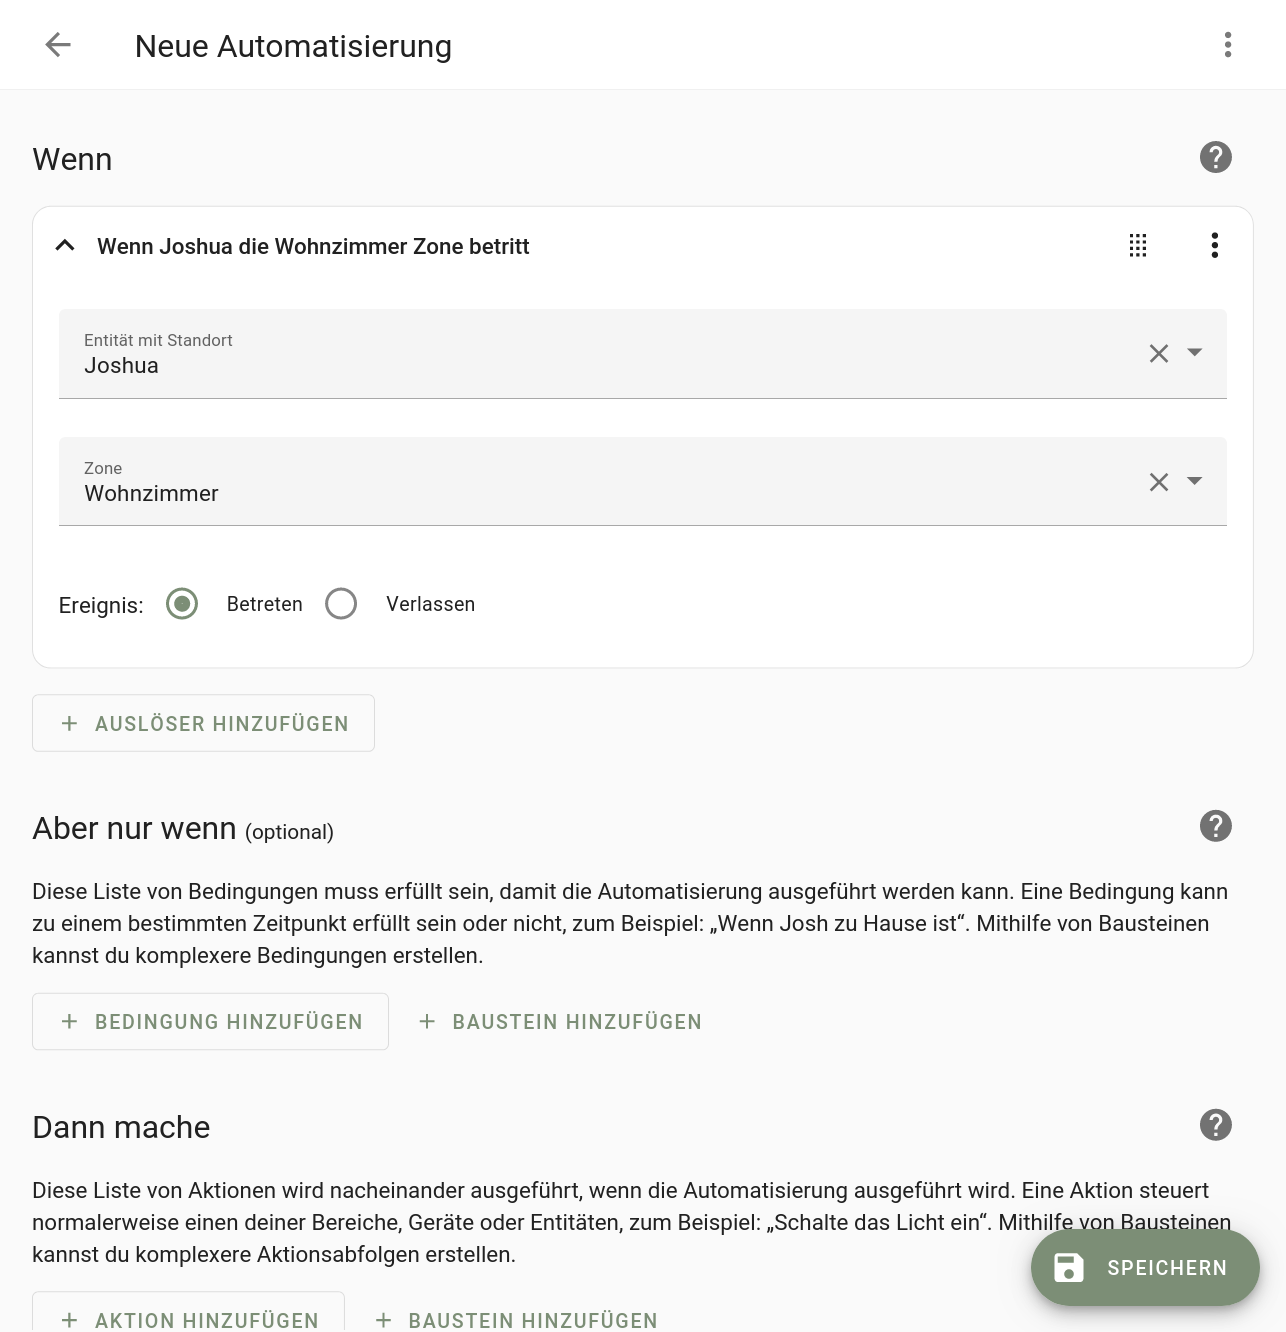
\includegraphics[width=\linewidth]{assets/hassio-automation-trigger.png}
    \caption[Angabe eines Auslösers in Home Assistant]{Angabe eines Auslösers in Home Assistant. Über Dropdown-Menüs und Radiobuttons können Einstellungen getroffen werden.}
    \label{fig:hassio-automation-trigger}
  \end{minipage}
  \hfill
  \begin{minipage}[t]{\hascwidth}
    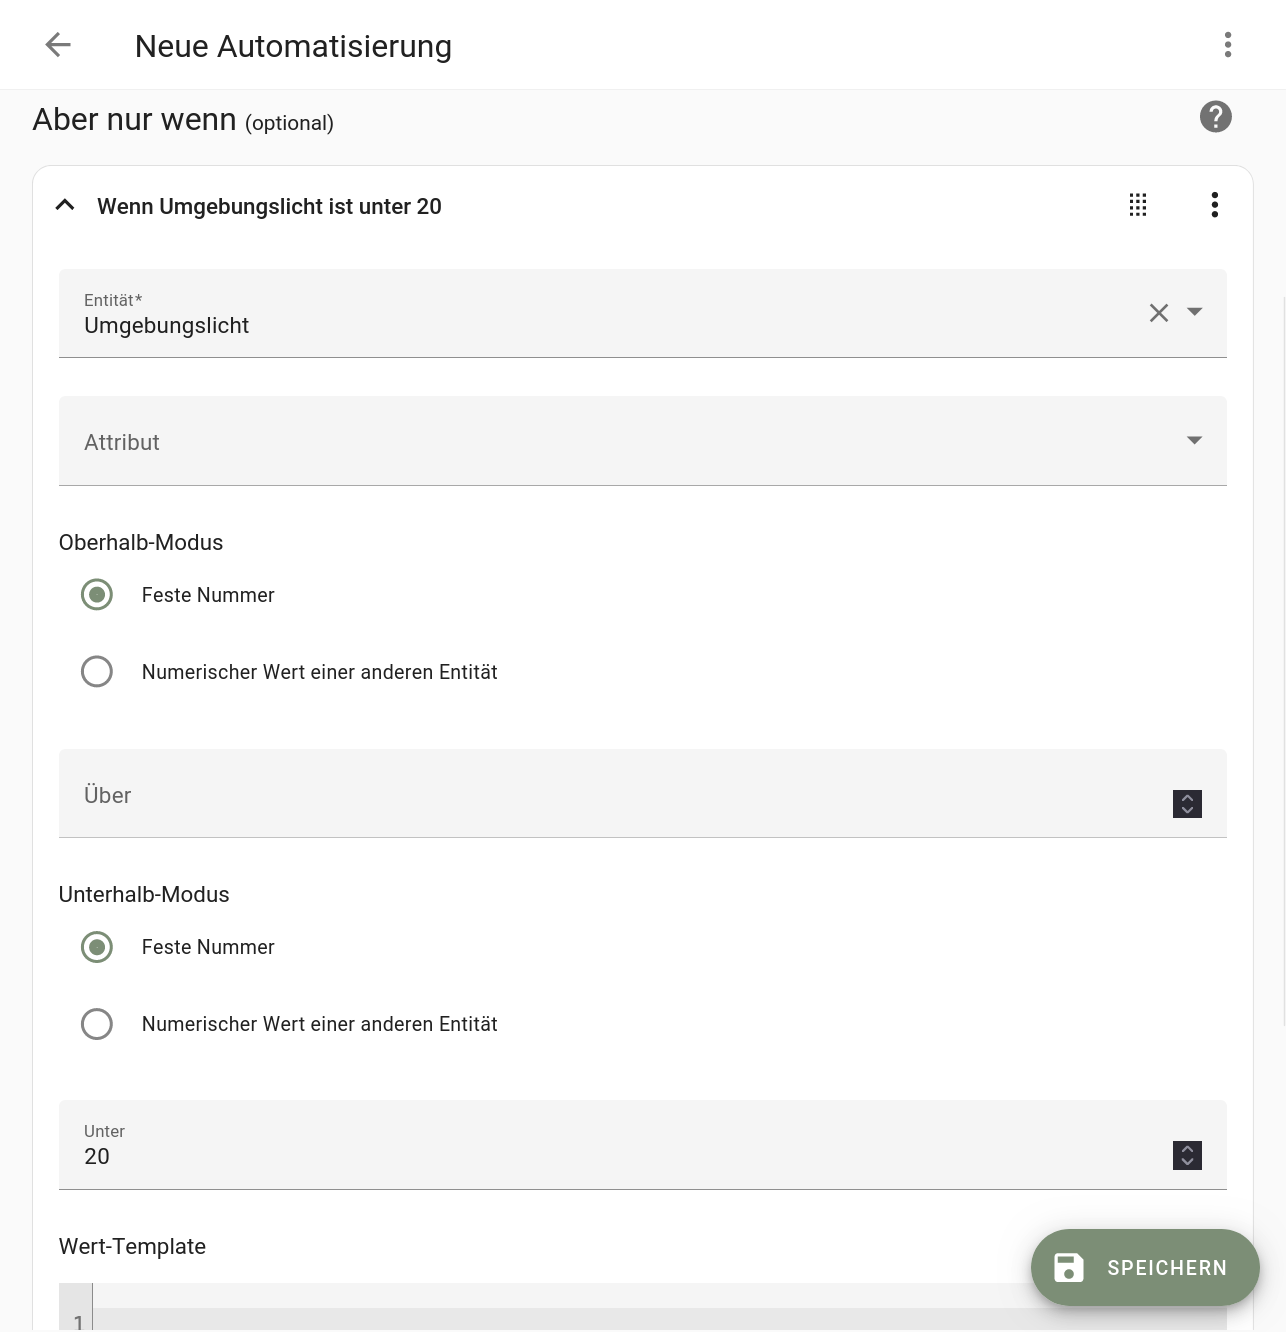
\includegraphics[width=\linewidth]{assets/hassio-automation-condition.png}
    \caption[Angabe einer Bedingung in Home Assistant]{Angabe einer Bedingung in Home Assistant. Je nach gewünschter Verhaltensweise können Angaben gemacht werden.}
    \label{fig:hassio-automation-condition}
  \end{minipage}
\end{figure}

Auf die gleiche Art und Weise können eine oder mehrere Aktionen hinzugefügt werden. Im vorliegenden Beispiel könnte dies eine Aktion sein, die die Entität "Leselampe" auf den Zustand "An" setzt. Komplexere Aktionsabläufe können über ein Pop-up-Fenster, welches Abbildung \ref{fig:hassio-automation-trigger-select-2} ähnelt, ausgewählt werden. Beispielsweise können Aktionen gleichzeitig ausgeführt werden, oder konditionale Strukturen gebildet werden \parencite{openhomefoundationScriptSyntax}.

Sobald ein Block definiert wurde, wird im Titel des Blocks eine natürlichsprachliche Zusammenfassung angezeigt, welche die im Block enthaltenen Elemente beschreibt. Dabei werden die gesetzten Variablen und getroffenen Auswahlen berücksichtigt. Zudem besteht die Möglichkeit, Blöcke einzuklappen, wodurch vertikaler Platz gespart wird.


Die erstellte Automatisierung wird als Datei im \ac{YAML}-Format gespeichert. Quelltext \ref{lst:automation} zeigt die durch die UI generierte \ac{YAML}-Datei. Die einzelnen Blöcke werden als Abschnitte (\texttt{trigger}, \texttt{condition}, \texttt{action}) abgespeichert und beinhalten die getroffenen Entscheidungen.

\lstinputlisting[
  label=lst:automation,
  caption={[\acs*{YAML}-Definition einer Automatisierung in Home Assistant]\acs*{YAML}-Definition einer Automatisierung in Home Assistant.},
  language=yaml,
  float=ht,
]{assets/hassio-automation.yaml}
